\documentclass[a0paper,portrait]{baposter}
%%%%%%%%%%%%%%%%%%%%%%%%%%%%%%%%%%%%%%%%%%%%%%%%
% Language, Encoding and Fonts
% http://en.wikibooks.org/wiki/LaTeX/Internationalization
%%%%%%%%%%%%%%%%%%%%%%%%%%%%%%%%%%%%%%%%%%%%%%%%
% Select encoding of your inputs. Depends on
% your operating system and its default input
% encoding. Typically, you should use
%   Linux  : utf8 (most modern Linux distributions)
%            latin1 
%   Windows: ansinew
%            latin1 (works in most cases)
%   Mac    : applemac
% Notice that you can manually change the input
% encoding of your files by selecting "save as"
% an select the desired input encoding. 
\usepackage[utf8]{inputenc}
% Make latex understand and use the typographic
% rules of the language used in the document.
\usepackage[english]{babel}
% Use the vector font Latin Modern which is going
% to be the default font in latex in the future.
\usepackage{helvet}
% Change the default font family from roman to sans serif
\renewcommand{\familydefault}{\sfdefault} % for text
% \usepackage[helvet]{sfmath} % for math
% Choose the font encoding
\usepackage[T1]{fontenc}
\usepackage{cite}
\usepackage{tikz}
\tikzset{>=latex}
\tikzstyle{block} = [draw,minimum size=0.5cm]
\usetikzlibrary{math,arrows,positioning,shapes.geometric, decorations.markings}
%%%%%%%%%%%%%%%%%%%%%%%%%%%%%%%%%%%%%%%%%%%%%%%%
% Graphics and Tables
% http://en.wikibooks.org/wiki/LaTeX/Importing_Graphics
% http://en.wikibooks.org/wiki/LaTeX/Tables
% http://pgfplots.sourceforge.net/
%%%%%%%%%%%%%%%%%%%%%%%%%%%%%%%%%%%%%%%%%%%%%%%%
% You cannot use floats in the baposter theme.
% We therefore load the caption package which provides
% the command \captionof
% Set up how figure and table captions are displayed
\usepackage{caption}
\captionsetup{
  font=small,% set font size to footnotesize
  labelfont=bf % bold label (e.g., Figure 3.2) font
}
% Make the standard latex tables look so much better
\usepackage{array,booktabs}
% For creating beautiful plots
\usepackage{pgfplots}
\usepackage[]{algorithm2e, setspace}
\newcommand\norm[1]{\left\lVert#1\right\rVert}
%%%%%%%%%%%%%%%%%%%%%%%%%%%%%%%%%%%%%%%%%%%%%%%%
% Mathematics
% http://en.wikibooks.org/wiki/LaTeX/Mathematics
%%%%%%%%%%%%%%%%%%%%%%%%%%%%%%%%%%%%%%%%%%%%%%%%
% Defines new environments such as equation,
% align and split 
\usepackage{amsmath}

% Adds new math symbols
\usepackage{amssymb}
\newenvironment{rcases}
  {\left.\begin{alignedat}{2}}
  {\end{alignedat}\right\rbrace}
  \DeclareMathOperator{\sgn}{sgn}
\let\oldtext\text
\renewcommand{\text}[1]{\oldtext{\fontfamily{ptm}\selectfont #1}}
\let\oldbf\textbf
\renewcommand{\textbf}[1]{\textcolor{aaublue1}{\oldbf{#1}}}

%%%%%%%%%%%%%%%%%%%%%%%%%%%%%%%%%%%%%%%%%%%%%%%%
% Colours
% http://en.wikibooks.org/wiki/LaTeX/Colors
%%%%%%%%%%%%%%%%%%%%%%%%%%%%%%%%%%%%%%%%%%%%%%%%
\selectcolormodel{RGB}
% define the three aau colors
\definecolor{aaublue1}{RGB}{33,26,82}% dark blue
\definecolor{aaublue2}{RGB}{113,109,143} % light blue
\definecolor{aaublue3}{RGB}{194,193,204} % lighter blue

%%%%%%%%%%%%%%%%%%%%%%%%%%%%%%%%%%%%%%%%%%%%%%%%
% Lists
% http://en.wikibooks.org/wiki/LaTeX/List_Structures
%%%%%%%%%%%%%%%%%%%%%%%%%%%%%%%%%%%%%%%%%%%%%%%%
% Easier configuration of lists
\usepackage{enumitem}
%configure itemize
\setlist{%
  topsep=0pt,% set space before and after list
  noitemsep,% remove space between items
  labelindent=\parindent,% set the label indentation to the paragraph indentation
  leftmargin=*,% remove the left margin
  font=\color{aaublue1}\normalfont, %set the colour of all bullets, numbers and descriptions to aaublue1
}
% use set<itemize,enumerate,description> if you have an older latex distribution
\setitemize[1]{label={\raise1.25pt\hbox{$\blacktriangleright$}}}
\setitemize[2]{label={\scriptsize\raise1.25pt\hbox{$\blacktriangleright$}}}
\setitemize[3]{label={\raise1.25pt\hbox{$\star$}}}
\setitemize[4]{label={-}}
%\setenumerate[1]{label={\theenumi.}}
%\setenumerate[2]{label={(\theenumii)}}
%\setenumerate[3]{label={\theenumiii.}}
%\setenumerate[4]{label={\theenumiv.}}
%\setdescription{font=\color{aaublue1}\normalfont\bfseries}

% use setlist[<itemize,enumerate,description>,<level>] if you have a newer latex distribution
%\setlist[itemize,1]{label={\raise1.25pt\hbox{$\blacktriangleright$}}}
%\setlist[itemize,2]{label={\scriptsize\raise1.25pt\hbox{$\blacktriangleright$}}}
%\setlist[itemize,3]{label={\raise1.25pt\hbox{$\star$}}}
%\setlist[itemize,4]{label={-}}
%\setlist[enumerate,1]{label={\theenumi.}}
%\setlist[enumerate,2]{label={(\theenumii)}}
%\setlist[enumerate,3]{label={\theenumiii.}}
%\setlist[enumerate,4]{label={\theenumiv.}}
%\setlist[description]{font=\color{aaublue1}\normalfont\bfseries}

%%%%%%%%%%%%%%%%%%%%%%%%%%%%%%%%%%%%%%%%%%%%%%%%
% Misc
%%%%%%%%%%%%%%%%%%%%%%%%%%%%%%%%%%%%%%%%%%%%%%%%
% change/remove some names
\addto{\captionsenglish}{
  %remove the title of the bibliograhpy
  \renewcommand{\refname}{\vspace{-0.7em}}
  %change Figure to Fig. in figure captions
  \renewcommand{\figurename}{Fig.}
}
% create links
\usepackage{url}
%note that the hyperref package is currently incompatible with the baposter class

%%%%%%%%%%%%%%%%%%%%%%%%%%%%%%%%%%%%%%%%%%%%%%%%
% Macros
%%%%%%%%%%%%%%%%%%%%%%%%%%%%%%%%%%%%%%%%%%%%%%%%
\newcommand{\alert}[1]{{\color{aaublue1}#1}}

%%%%%%%%%%%%%%%%%%%%%%%%%%%%%%%%%%%%%%%%%%%%%%%%
% Document Start 
%%%%%%%%%%%%%%%%%%%%%%%%%%%%%%%%%%%%%%%%%%%%%%%%
\begin{document}
%%%%%%%%%%%%%%%%%%%%%%%%%%%%%%%%%%%%%%%%%%%%%%%%
% Some changes that cannot be made in the preamble
%%%%%%%%%%%%%%%%%%%%%%%%%%%%%%%%%%%%%%%%%%%%%%%%
% set the background of the poster
\background{
  \begin{tikzpicture}[remember picture,overlay]%
    %the poster background color
    \fill[fill=aaublue3] (current page.north west) rectangle (current page.south east);
    %the header
    \fill [fill=aaublue1] (current page.north west) rectangle ([yshift=-\headerheight] current page.north east);
  \end{tikzpicture}
}
% if you want to reduce the space before and after equations, use and adjust
% the following lines
%\addtolength{\abovedisplayskip}{-2mm}
%\addtolength{\belowdisplayskip}{-2mm}

%%%%%%%%%%%%%%%%%%%%%%%%%%%%%%%%%%%%%%%%%%%%%%%%
% General poster setup
%%%%%%%%%%%%%%%%%%%%%%%%%%%%%%%%%%%%%%%%%%%%%%%%
\begin{poster}{
  %general options for the poster
  grid=false,
  columns=3,
%  colspacing=4.2mm,
  headerheight=0.1\textheight,
  background=user,
%  bgColorOne=red!42, %is used when background != user and none
%  bgColortwo=green!42, %is used when background is shaded
  eyecatcher=true,
  %posterbox options
  headerborder=closed,
  borderColor=aaublue1,
  headershape=rectangle,
  headershade=plain,
  headerColorOne=aaublue1,
%  headerColortwo=yellow!42, %is used when the header background is shaded
  textborder=rectangle,
  boxshade=plain,
  boxColorOne=white,
%  boxColorTwo=cyan!42,%is used when the text background is shaded
  headerFontColor=white,
  headerfont=\Large\sf\bf,
  linewidth=1pt
}
%the Eye Catcher (the logo on the left)
{
  %this can be commented out or replaced by a company/department logo
  
\includegraphics[height=0.75\headerheight]{AAUgraphics/aau_logo_new_neg}
}
%the poster title
{\color{white}\bf \Large
  Real-time Implementation of an Elasto-Plastic Friction Model applied to Stiff Strings using Finite-Difference Schemes
}
%the author(s)
{\color{white}\small
  \vspace{1em} Silvin Willemsen$^\oldtext{1}$, Stefan Bilbao$^\oldtext{2}$, Stefania Serafin$^\oldtext{1}$\\[0.5em]
  $^\oldtext{1}$ Multisensory Experience Lab, CREATE, Aalborg University Copenhagen, Denmark\\
  $^\oldtext{2}$ Acoustics and Audio Group, University of Edinburgh, UK \\
  sil@create.aau.dk
}
%the logo (the logo on the right)
{
  %this can be commented out or replaced by a company/department logo
  
\includegraphics[height=0.75\headerheight]{melablogo.png}
}

%%%%%%%%%%%%%%%%%%%%%%%%%%%%%%%%%%%%%%%%%%%%%%%%
% the actual content of the poster begins here
%%%%%%%%%%%%%%%%%%%%%%%%%%%%%%%%%%%%%%%%%%%%%%%%

\begin{posterbox}[name=intro,column=0,row=0]{Introduction}
\begin{itemize}
    \item The simulation of a \textbf{bowed string} is challenging due to the strongly \textbf{non-linear relationship} between the bow and the string.
    \item This relationship can be described by a \textbf{model of friction}.
    \item A recently popular and accurate friction model is the \textbf{elasto-plastic} model.
    \item This can be applied to a string implemented with \textbf{FDTD methods}, which are also focused on accuracy. 
    \item We are interested in \textbf{bridging the gap} between highly \textbf{accurate} physical models and \textbf{efficient} implementations. \item In this work, we present an implementation of the elasto-plastic friction model in conjunction with a finite-difference implementation of the damped stiff string. 
    \item Furthermore, we show that it is possible to play the string in \textbf{real-time} using the Sensel Morph controller \cite{Sensel2019}.
\end{itemize}
\end{posterbox}

\begin{posterbox}[name=elasto,column=0,below=intro, above=bottom]{Elasto-Plastic Bow Model}
\begin{itemize}

    \item The elasto-plastic friction model assumes that the friction between objects in contact is caused by a large \textbf{ensemble of bristles} (see Fig. \ref{fig:elasto}). 
    \item Next to the relative velocity $v$ between the bow and the string, the \textbf{average bristle displacement} $z$ is introduced as a second independent variable. 
\end{itemize}
\begin{center}
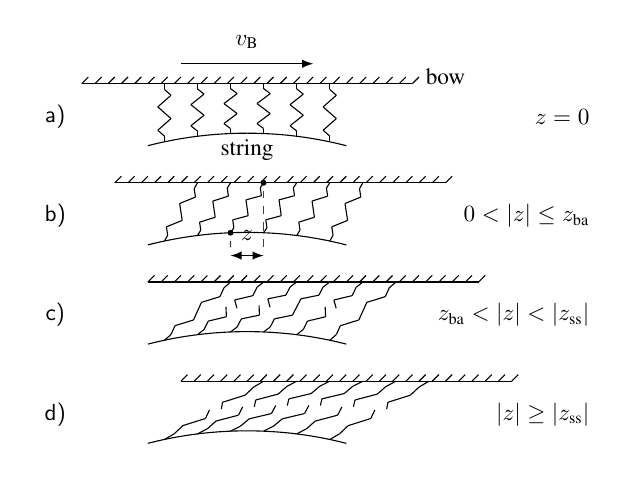
\begin{tikzpicture}[scale=0.84, every node/.style={transform shape}]
    
    \def\radius{6}; % Radius of the string (>2!)
    \pgfmathsetmacro{\reps}{3}; % How may back-and-forths in the drawing of the springs
    \def\horShift{0.5}; %how far the bow is shifted to the right in b)
    \def\bowSpacing{0.2};
    \def\drawingSpacing{1.5};
    \def\bowWidth{5};
    \def\descDist{5.3};
    %subfigure letters
    \node (nothing) at (-3.2, 0.5 - \drawingSpacing) {};
    \node (A) at (-2.9, 0.5) {a)};
    \node (B) at (-2.9, 0.5 - \drawingSpacing) {b)};
    \node (C) at (-2.9, 0.5 - \drawingSpacing * 2) {c)};
    \node (D) at (-2.9, 0.5 - \drawingSpacing * 3) {d)};
    
    %bow velocity arrow
    \draw[->] (-1, 1.3) -- (1, 1.3) node [midway, above = 0.1cm] (velText) {$v_\text{B}$};
    
    \pgfmathsetmacro{\zCoordTop}{0};
    \pgfmathsetmacro{\zYCoordBottom}{0};
    \def\springForZ{2}
    \foreach \drawing in {0, ..., 3}
    {
        %% Draw String
        \begin{scope}
            \clip (-1.5,-0.2- \drawing * \drawingSpacing) rectangle (1.5,1.5);
            \draw (0,-\radius + 0.25 - \drawing * \drawingSpacing) circle(\radius);
        \end{scope}

        %% Draw Bow
        \def\halfBW{\bowWidth*0.5}
        \pgfmathsetmacro{\halfNumDiag}{0.5 * \bowWidth / \bowSpacing};
        \draw[-] (-\halfBW + \drawing * \horShift,1 - \drawing * \drawingSpacing) -- (\halfBW + \drawing * \horShift, 1 - \drawing * \drawingSpacing);
        \foreach \bowDiag in {-\halfNumDiag, ...,\halfNumDiag}
        {
        \pgfmathtruncatemacro{\bD}{\bowDiag}
        % \ifnum\drawing=0
        %     \ifnum\bD<-1
        %         \draw[-] (\drawing * \horShift + \bowDiag * \bowSpacing, -\drawing * \drawingSpacing + 1) -- (\drawing * \horShift + \bowDiag * \bowSpacing + 0.1, -\drawing * \drawingSpacing + 0.1 + 1);
        %         \else
        %         \ifnum\bD>1
        %             \draw[-] (\drawing * \horShift + \bowDiag * \bowSpacing, -\drawing * \drawingSpacing + 1) -- (\drawing * \horShift + \bowDiag * \bowSpacing + 0.1, \drawing * -2 + 0.1 + 1);
        %         \fi
        %     \fi
        % \else
            \draw[-] (\drawing * \horShift + \bowDiag * \bowSpacing, -\drawing * \drawingSpacing + 1) -- (\drawing * \horShift + \bowDiag * \bowSpacing + 0.1, -\drawing * \drawingSpacing + 0.1 + 1);
        % \fi
            
        }
        
        \def\brokenSprings{{0, 1, 1, 0, 1, 0}};
        %% Draw Springs
        \foreach \springNo in {0, ..., 5}
        {
            % Calculate spring length depending on the radius of the string
            \pgfmathsetmacro{\startX}{\springNo  * 0.5 - 1.25};
            \pgfmathsetmacro{\calcSpace}{(\radius + 1) - \radius * sin(acos(\startX/\radius)) - 0.25};
            \pgfmathsetmacro{\springLength}{sqrt(\calcSpace*\calcSpace+\drawing*\horShift*\drawing*\horShift)};
            
            \pgfmathsetmacro{\spacing}{\springLength / (\reps + 2)}; 
            % spacing between two spring-back-and-forths
            \ifnum\drawing=0
                \pgfmathsetmacro{\rot}{0};
            \else
                \pgfmathsetmacro{\rot}{(270+(atan(\calcSpace/(\drawing*\horShift))))}; %rotation of the springs
            \fi
            
            \ifnum\drawing=1
                \ifnum\springNo=\springForZ
                    \pgfmathsetmacro{\resTwo}{sqrt(\springLength*\springLength-\horShift*\horShift)};
                    \global\let\zCoordBottom = \resTwo;
                \fi
            \fi
        
            \pgfmathsetmacro{\isBroken}{\brokenSprings[\springNo]};
            % debug code
            % \node (nodeTest\springNo) at (\springNo*1.1-2, -3 - 1 * \drawing + 0.3 * \springNo) {\isBroken};
            
            \begin{scope}[shift={(\startX + \drawing * \horShift,1 -\drawing * \drawingSpacing)}]
                \pgfmathsetmacro{\xWidth}{0.1 - (\drawing * 0.02)};
                \draw[-, rotate = \rot] (0, 0) -- (0, -\spacing * 0.5);
                \draw[-, rotate = \rot] (0, -\spacing * 0.5) -- (\xWidth, -\spacing);
                \def\Y{-\spacing}
                \foreach \idx in {1,...,\reps}
                {
                    \pgfmathsetmacro{\idxMinOne}{\idx-1};
                    \ifnum\drawing=2
                        \ifnum\isBroken=1
                            \pgfmathtruncatemacro{\idxT}{\reps * 0.5 + 1}
                            \ifnum\idx=\idxT
                                \draw[-, rotate = \rot] (\xWidth, \Y - \idxMinOne * \spacing) -- (-\xWidth,\Y - \idx * \spacing*0.6);
                                \draw[-, rotate = \rot] (\xWidth, \Y - \idxMinOne * \spacing * 1.66) -- (-\xWidth,\Y - \idx * \spacing);
                            \else
                                \draw[-, rotate = \rot] (\xWidth, \Y - \idxMinOne * \spacing) -- (-\xWidth,\Y - \idx * \spacing);
                            \fi
                        \else
                                \draw[-, rotate = \rot] (\xWidth, \Y - \idxMinOne * \spacing) -- (-\xWidth,\Y - \idx * \spacing);
                        \fi
                    \else
                        \ifnum\drawing=3
                            \pgfmathtruncatemacro{\idxT}{\reps * 0.5 + 1}
                            \ifnum\idx=\idxT
                                \draw[-, rotate = \rot] (\xWidth, \Y - \idxMinOne * \spacing) -- (-\xWidth,\Y - \idx * \spacing*0.6);
                                \draw[-, rotate = \rot] (\xWidth, \Y - \idxMinOne * \spacing * 1.66) -- (-\xWidth,\Y - \idx * \spacing);
                            \else
                                \draw[-, rotate = \rot] (\xWidth, \Y - \idxMinOne * \spacing) -- (-\xWidth,\Y - \idx * \spacing);
                            \fi
                        \else
                            \draw[-, rotate = \rot] (\xWidth, \Y - \idxMinOne * \spacing) -- (-\xWidth,\Y - \idx * \spacing);
                        \fi
                    \fi
                    \pgfmathsetmacro{\invXWidth}{\xWidth*-1};
                    \global\let\xWidth = \invXWidth;
                    \pgfmathsetmacro{\lastYPre}{\Y - \idx * \spacing};
                    \global\let\lastY = \lastYPre;
                }
                \draw[-, rotate = \rot] (\xWidth, \lastY) -- (0, \lastY - \spacing * 0.5);
                \draw[-, rotate = \rot] (0, \lastY - \spacing * 0.5) -- (0, \lastY - \spacing);
             \end{scope}
             
        }
        % \draw[<->] (2,2-0.707) -- node[right] {$r=\sqrt{2} \Rightarrow A=\pi(\sqrt{2})^2=2\pi$} (2,2+0.707);
        
        % \node(stringText) at (0, -\drawing * 2) {string};
        % \node[block, minimum height = 0.15cm, fill=white, draw=white] (bowText) at (\drawing * \horShift, 1.23 - \drawing * 2) {bow};
    }
    \filldraw[black] (-1.25+\springForZ*0.5 + \horShift,1-\drawingSpacing) circle (1pt) node[anchor=center](topZ){};
    \filldraw[black] (-1.25++\springForZ*0.5,1-\zCoordBottom-\drawingSpacing) circle (1pt) node[anchor=center](bottomZ){};
    
    \node [](leftNode) at (-1.25+\springForZ*0.5,-\drawingSpacing - 0.1) {};
    \node [](rightNode) at (-1.25 +\springForZ*0.5 + \horShift,-\drawingSpacing - 0.1) {};
    
    \draw[<->] (leftNode.center) -- (rightNode.center) node [midway, above = 0.1cm] (TextNode) {$z$};
    \draw[dashed, darkgray] (leftNode) -- (bottomZ);
    \draw[dashed, darkgray] (rightNode) -- (topZ);
    %% Draw bow and string texts
        \node(stringText) at (0, 0) {$\text{string}$};
        \node(bowText) at (3, 1.1) {$\text{bow}$};
    %% Draw descriptions of z
    \def\zTexts{{"$z=0$", "$0<|z|<z_{\text{ba}}$", "$z_{\text{ba}}<|z|< z_\text{ss}$", "$|z|>z_\text{ss}$"}};
    
    \node[anchor = east](zText1) at (\descDist, 0.5) {$z=0$};
    \node[anchor = east](zText1) at (\descDist, 0.5 - \drawingSpacing) {$0<|z|\leq z_{\text{ba}}$};
    \node[anchor = east](zText1) at (\descDist, 0.5 - \drawingSpacing * 2) {$z_{\text{ba}}<|z|< |z_\text{ss}|$};
    \node[anchor = east](zText1) at (\descDist, 0.5 - \drawingSpacing * 3) {$|z|\geq|z_\text{ss}|$};
    
    \end{tikzpicture}
    \captionsetup{singlelinecheck=off}
    \captionof{figure}[f]{%\it \fontfamily{ptm}\selectfont 
    Microscopic displacements of the bristles between the bow and the string. The bow moves right with a velocity of $v_\text{B}$.
    \begin{enumerate}[labelindent=-2.4pt, label=\alph*), font=\color{black}]
        \item \textbf{Initial} state. The average bristle displacement $z=0$.
        \item The purely \textbf{elastic}, or presliding regime (STICK).
        \item The \textbf{elasto-plastic} regime. 
        \item The purely \textbf{plastic} regime (SLIP).
    \end{enumerate}
}
    \label{fig:elasto}
    \end{center}
    \hrule
    \vspace{0.2cm}
    {\large \textbf{Applying to stiff string}}\\
    % \begin{itemize}
    %     \item 
        Using the subscripts $t$ and $x$ to denote differentiation, we can write the equation for the bow-excited \textbf{linear damped stiff string}
    % \end{itemize}
    \begin{equation}
\begin{aligned}\label{eq:stiffString}
  u_{tt} = &\, c^2u_{xx}-\kappa^2u_{xxxx}-2\sigma_0u_t+2\sigma_1u_{txx}\\
  &-\delta(x-x_\text{B})f(v,z)/\rho A
  \end{aligned}
\end{equation}
% \begin{itemize}
%     \item[] 
with \textbf{force function}
% \end{itemize}
\vspace{0.1cm}
\begin{equation}
    f(v,z) = s_0z+s_1\dot{z}+s_2v+s_3w,
\end{equation}
% \begin{itemize}
    % \item[] 
    and \textbf{relative velocity} with bowing point $x_\text{B}$ and bowing velocity $v_\text{B}$ is defined as
% \end{itemize}
\begin{equation}
    v = u_t(x_\text{B})-v_\text{B}.
\end{equation}

\end{posterbox}

\begin{posterbox}[name=elasto2, column=1, row=0]{Elasto-Plastic Bow Model cont.}
The \textbf{time-derivative of $z$} is defined as $\dot{z}$ and is related to $v$ through
\begin{equation}\label{eq:zdot}
    \dot{z} = r(v,z) = v\left[1-\alpha(v,z)\frac{z}{z_\text{ss}(v)}\right],
\end{equation}
with \textbf{steady-state function} $z_\text{ss}$ (see Fig. \ref{fig:steadyState}),
% \begin{equation}
%     z_\text{ss}(v)=\frac{\sgn(v)}{s_0}\left[f_\text{C}+(f_\text{S}-f_\text{C})e^{-(v/v_\text{S})^2}\right]\; .
% \end{equation}
\begin{center}
  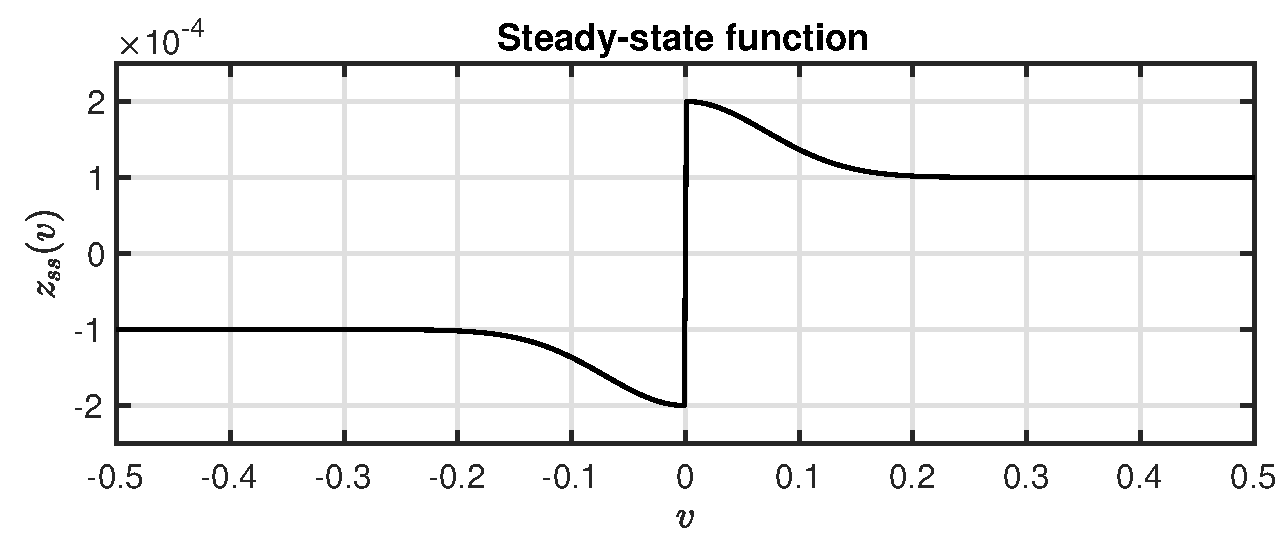
\includegraphics[width=0.95\columnwidth]{steadyState.eps}
  \captionof{figure}{A plot of the steady-state function $z_\text{ss}(v)$ with a force of 5 N.}
  \label{fig:steadyState}
\end{center}

and the \textbf{adhesion map} between the bow and the string $\alpha(v,z)$, which is defined as (see Fig. \ref{fig:alpha})
\vspace{-1em}
\begin{equation}
    \alpha(v, z) = 
% \begin{aligned}
    \begin{cases}
    \begin{rcases}
        &0 & |z| \leq z_\text{ba}\\
       &\alpha_\text{m}&\ \, z_\text{ba}<|z|<|z_\text{ss}(v)|\\        &1 &|z|\geq|z_\text{ss}(v)|
        \end{rcases} 
        
         \ \text{if} \ \ \begin{gathered}
          \sgn(v)\\[-1ex]
          =\\[-1.05ex]
          \sgn(z)
        \end{gathered}  \\[3ex]
        \; \!0%\!\!\!\!\!\!\,
        \qquad\qquad\qquad\; \text{if}\, \: \sgn(v)\neq\sgn(z)
    \end{cases}
    % \end{aligned}
    \nonumber
\end{equation}
where $\alpha_m$ is the transition between the elastic and plastic behaviour.
% and the transition between the elastic and plastic behaviour is defined as
% \begin{align}
%     \alpha_\text{m} &= \frac{1}{2}\big[1+\sgn(z)\sin(\Psi)\big]\\
%     \text{where} \quad \Psi &= \pi\frac{z-\sgn(z)\frac{1}{2}(|z_\text{ss}(v)|+z_\text{ba})}{|z_\text{ss}(v)|-z_\text{ba}}\nonumber\, .
%     \end{align}
    \begin{center}
  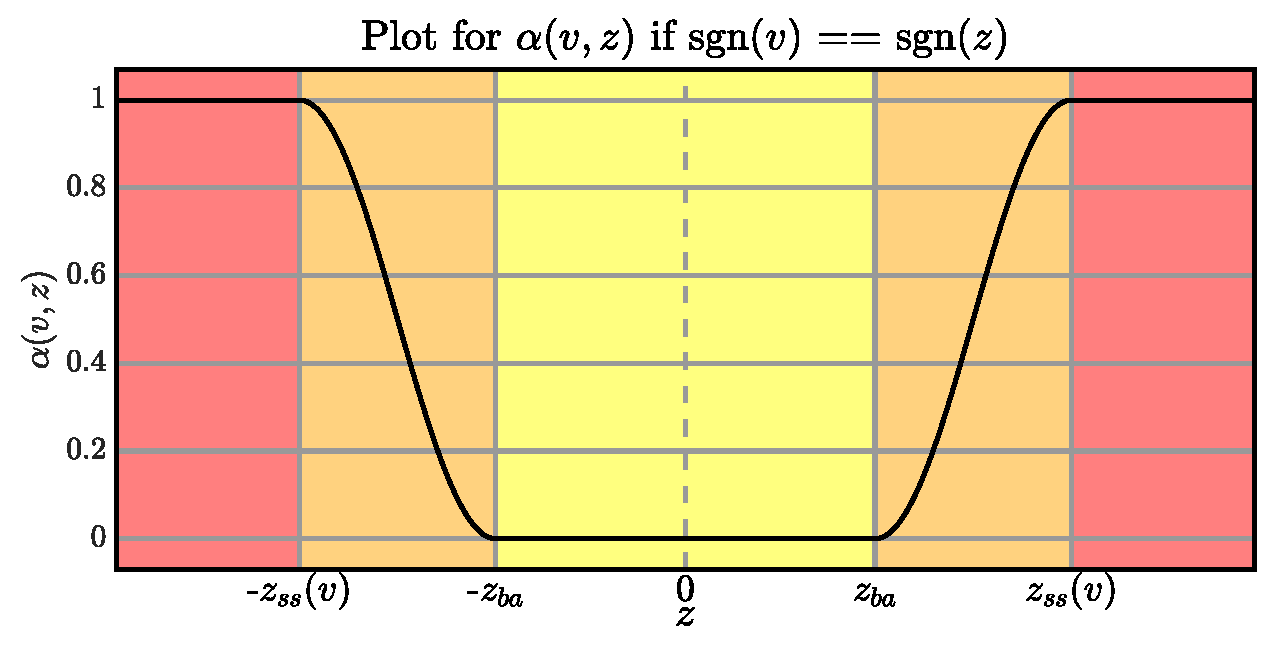
\includegraphics[width=0.95\columnwidth]{drawAlpha3.eps}
  \captionof{figure}{A plot of the adhesion map $\alpha(v,z)$ plotted against $z$ when the signs of $v$ and $z$ are the same. The different regions of the map are shown with the coloured areas and correspond to Fig. \ref{fig:elasto} according to: yellow - a) \& b), orange - c) and red - d).}
  \label{fig:alpha}
\end{center}
\end{posterbox}

% \begin{posterbox}[name=equation,column=0,below=elasto2]{Equations}
% Here is an example of an equation
% \begin{equation}
% \begin{aligned}
%   u_{tt} = &\, c^2u_{xx}-\kappa^2u_{xxxx}-2\sigma_0u_t+2\sigma_1u_{txx}\\
%   &-\delta(x-x_\text{B})f(v,z)/\rho A.
%   \end{aligned}
% \end{equation}
% with force function
% \begin{equation}
%     f(v,z) = s_0z+s_1\dot{z}+s_2v+s_3w
% \end{equation}
% \end{posterbox}
% \begin{posterbox}[name=parameters,column=1,below=elasto2,above=bottom]{Parameter values}
% \begin{center}
%   \captionof{table}{Parameter values used for the simulation.}
% 	\centering
%   \begin{tabular}{c|c|c}
%     Parameter & Symb. & Value\\ \hline
%     Material Density &$\rho$ & $7850$ \\
%     Radius & $r$ & $5\cdot10^{-4}$\\
%     String length & $L$ & $1$ \\
%     Wave speed & $c$ & $2 f_0/L$\\
%     Young's modulus & $E$ & $2\cdot 10^{11}$\\
%     Freq. ind. damping & $\sigma_0$ & $1$\\
%     Freq. dep. damping & $\sigma_1$ & $5 \cdot 10^{-3}$\\
%     Coulomb friction & $\mu_\text{C}$ & $0.3$ \\
%     Static friction & $\mu_\text{S}$ & $0.8$ \\
%     Normal force & $f_\text{N}$ & $10$ \\
%     Bow velocity & $v_\text{B}$ & $0.1$ \\
%     Bow position & $x_\text{B}$ & $0.25$ \\
%     Stribeck velocity & $v_\text{S}$ & $0.1$ \\
%     Bristle stiffness & $s_0$ & $10^4$ \\
%     Bristle damping & $s_1$& $0.001\sqrt{s_0}$ \\
%     Viscous friction & $s_2$ & $0.4$ \\
%     Noise coefficient & $s_3$ & $0.02f_\text{N}$\\
%     Pseudorand. func. & $w$ & $-1<w<1$\\
%     Break-away disp.& $z_\text{ba}$ & $0.7 f_\text{C}/s_0$ \\
%     Sample rate & $f_\text{s}$ & $44,100$ \\
%     Time step & $k$ & $1/f_\text{s}$ \\
%     %NR threshold & $\phi$ (-) & $10^{-7}$ \\
%  \end{tabular}
% 	%
%   \label{tab:parameters}
% \end{center}
% \end{posterbox}

\begin{posterbox}[name=discretisation, column=1, below=elasto2,above=bottom]{Discretisation}
% \begin{itemize}
%     \item 
    At the bowing point we need to iteratively solve for relative velocity $v^n$ and average bristle displacement $z^n$ at sample $n$ using \textbf{multivariate Newton-Raphson}.
    % \item
    We can rewrite \eqref{eq:stiffString} (in discrete-time) to
    % \end{itemize}
    \vspace{-0.3em}
    \begin{equation}
    \begin{aligned}
        g_1(v^n, z^n) = \, &\frac{s_0z^n+s_1r^n+s_2v^n+s_3w^n}{\rho A h}
    \\&+\Big(\frac{2}{k} + 2\sigma_0 \Big)v^n
    + b^n= 0,
    \end{aligned}\vspace{-0.2em}
    \end{equation}
    where $b^n$ is not dependent on $v^n$ and $z^n$ and can be pre-computed. Furthermore, using the \textbf{discrete counterpart of \eqref{eq:zdot}} and defining $a^n$ as the \textbf{trapezoid rule applied to $z$}, we define
    \vspace{-0.3em}\begin{equation}
        g_2(v^n, z^n) = r^n - a^n ,
        \vspace{-0.3em}
    \end{equation}
    and obtain the following iteration
    \begin{equation}\label{eq:NRit}
    \begin{bmatrix}
    v_{(i+1)}^n\\
    z_{(i+1)}^n
    \end{bmatrix}
    =
    \begin{bmatrix}
    v_{(i)}^n\\
    z_{(i)}^n
    \end{bmatrix}
    -
    \begin{bmatrix}
    \frac{\partial g_1}{\partial v} & \frac{\partial g_1}{\partial z}\\
    \frac{\partial g_2}{\partial v} & \frac{\partial g_2}{\partial z}\\
    \end{bmatrix}^{-1}
    \begin{bmatrix}
    g_1\\
    g_2
    \end{bmatrix}
    ,
\end{equation}
where $i$ is the iteration number capped by 50 iterations, and the convergence threshold is set to $10^{-7}$.

\end{posterbox}

\begin{posterbox}[name=implementation,column=2,row=0]{Implementation}

\begin{itemize}
    \item The real-time implementation has been done using \textbf{C++} and the \textbf{JUCE} framework \cite{JUCE}.
\end{itemize}
\begin{center}
    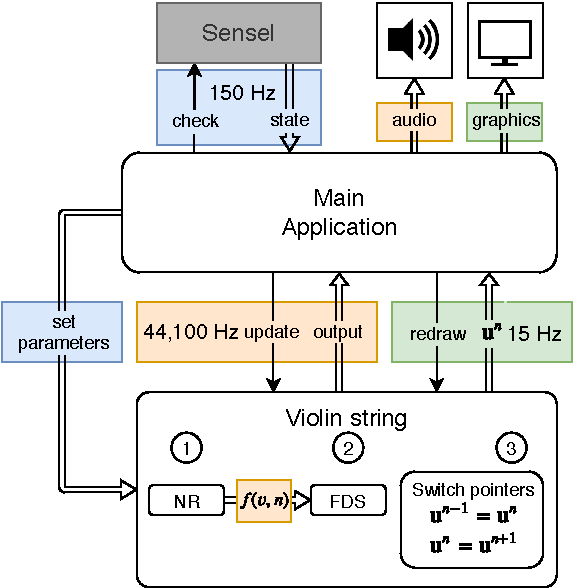
\includegraphics[width=1.0\columnwidth]{systemArchitecture.pdf}
    \captionof{figure}{The system architecture. Black arrows indicate instructions and hollow arrows indicate data flows. %Arrows are accompanied by coloured boxes depicting what thread they are associated with.
    }
    \label{fig:systemArch}
\end{center}
\begin{itemize}
    \item The three main \textbf{components} of the application are:
    \begin{itemize}
        \item the \textbf{Sensel} for controlling the application,
        \item the \textbf{violin string class} that performs the simulation, and
        \item the \textbf{main application class} that moderates between these and the auditory and visual outputs.
    \end{itemize}
    \item The three main threads running are (color in Fig. \ref{fig:systemArch}, frequency):
    \begin{itemize}
        \item the \textbf{Graphics} thread (green, 15 Hz)
        \item the \textbf{Sensel} thread (blue, 150 Hz)
        \item the \textbf{Audio} thread (orange, 44,100 Hz)
    \end{itemize}
\end{itemize}
\end{posterbox}

\begin{posterbox}[name=discussion,column=2,below=implementation]{Results and Discussion}
\begin{itemize}
    \item The algorithm was tested with different numbers of strings according to the violin tuning of empty strings. 
\end{itemize}
\vspace{-1.6em}
  \begin{center}
  \captionof{table}{Average CPU usage for different amounts of strings. All strings are bowed simultaneously (polyphonically).}
	\centering
  \begin{tabular}{|c|c|c|}\hline
   
   \# strings & Graphics (\%) & No graphics (\%)\\
    \hline
    1 & 44.8 & 5.95\\
    2 & 47.7 & 9.54\\
    3 & 52.8 & 12.1 \\
    4 & 60.9 & 17.9\\
    \hline
 \end{tabular}
	%
  \label{tab:results}
\end{center}
\end{posterbox}

\begin{posterbox}[name=conclusion,column=2,below=discussion]{Conclusion}
  \begin{itemize}
    \item With a single string we are able to keep the \textbf{CPU usage under 6$\mathbf{\%}$}.
    % \item This implementation could thus easily be used in parallel with other virtual instruments or plugins.
    \item Future work includes parameter design and including an instrument body for a more realistic sound. 
  \end{itemize}
\end{posterbox}

% \begin{posterbox}[name=feedback,column=2,below=problems]{Feedback}
%   \begin{itemize}
%     \item The AAU poster theme has been tested with baposter v. 2.0, and it can be downloaded from my Github-site \cite{jkngithub}.
%     \item If you find a bug in the AAU theme (and not in the baposter template), please do not hesitate to contact me. There is a FAQ at the baposter website \cite{baposter}, if you should have any problems with it.
%   \end{itemize}
% \end{posterbox}

\begin{posterbox}[name=refs,column=2, below=conclusion,above=bottom]{References}
% In the last box, you will usually have a list of references
% The bibliography automatically adds the title "References", but
% this have been removed in the preamble

% use either ......
% \bibliographystyle{plain}
% \begin{thebibliography}{1}% Simple bibliography with widest label of 1
% \itemsep=-0.01em% Save space between the separation
% \setlength{\baselineskip}{0.4em}% Save space with longer lines
% \bibitem{JUSE} Brian Amberg: \emph{LaTeX Poster Template}, \url{http://www.brian-amberg.de/uni/poster/} 
% \bibitem{pgfplots} Christian Feuersänger: \emph{PGFPlots - A LaTeX Package to create normal/logarithmic plots in two and three dimensions}, \url{http://pgfplots.sourceforge.net/} 
% \bibitem{jkngithub} Jesper Kjær Nielsen: \emph{Official AAU Beamer Theme, Poster Theme, and Report Template}, \url{http://github.com/jkjaer/aauLatexTemplates}
% \bibitem{ctan} The CTAN Team  \emph{sfmath -  Sans-serif mathematics}, \url{http://ctan.org/pkg/sfmath}
% \end{thebibliography}


% ...... or
 \bibliographystyle{IEEEbib}
 \bibliography{mybib} 
\end{posterbox}

\end{poster}
\end{document}
